\chapter*{Introduction}
\markboth{Introduction}{Introduction}
\addcontentsline{toc}{chapter}{Introduction}
\chapterimage
\thispagestyle{plain}

\begin{multicols*}{2}
Dark Dungeons is a Role-Playing Game. This book contains the rules of the game.

\section{What is a Role-Playing Game?}
Role-playing games have been around since the mid 1970s.

When they first started, they had their roots in war-gaming (moving model armies around in simulation of historical battles) and descriptions of role-playing games would have used those war games, along with such childhood games as “Cops and Robbers” and “Cowboys and Indians” as reference points.

However, now that were in the second decade of the 21st century, times – and cultural reference points – have changed.

For most people today, the term “role playing game” is usually found abbreviated to “RPG” and is usually preceded by the letters “C” (becoming “CRPG” or “Computer Role Playing Game”) or “MMO” (becoming “MMORPG” or “Massively Multiplayer Online Role Playing Game”).

In this genre of computer games, the player takes on the role of a character in an ongoing storyline – usually the main protagonist of the story.

The game consists of trying to get the story to progress towards its climax, often involving combat and problem solving.

Table-top role-playing games like Dark Dungeons have a similar basis, except that the game is controlled by a human Game Master rather than by a computer, and rather than the action taking place on a computer screen the action takes place in the imaginations of the players.

While this may sound like a step backwards at first glance, it is much more flexible and adaptable. On a CRPG, you are limited to telling the single story that the game designers wrote. You can’t go “off the map”. In a table-top role-playing game, however, you are not limited to fixed stories. The Game Master and the players can between them create an infinite number of stories, limited only by their imaginations. The Game Master can create whatever scenarios and situations they want to, and the players are not constrained to only doing what has been anticipated.

If they want their characters to do something, they don’t have to simply hope that some designer wrote it into the game. They simply tell the Game Master what their character is trying to do and the Game Master can improvise in a way that a computer never could (although the rules and guidelines in this book cover most common situations so that they can be handled in a consistent manner).

The other main difference between a table-top role-playing game and a CRPG is the social aspect. Although many CRPGs allow the player to control a whole party of characters rather than just a single one, they are still largely solitary affairs. Table-top role-playing games are generally designed for groups of players to play together and Dark Dungeons is no exception. Although it can be played with only a single player and a Game Master, it plays best with 3-8 players playing together, each controlling a single character. Interaction between the characters controlled by the different players, as well as non-scripted interaction between the characters controlled by players and characters controlled by the Game Master, is one of the chief elements of a table-top role-playing game.

\section{What Do You Need to Play?}
The only things that are needed to play are pencils, paper and dice.

\subsection{Dice}
In Dark Dungeons, dice will be needed to resolve a lot of situations where the whims of fortune have an effect on the outcome of a situation. As well as the traditional cubic dice numbered from one to six, the game uses a variety of other dice of different shapes. Since these each have different numbers of sides, they are often called polyhedral dice.

If you have already played other role playing games, you may already own some of these dice. If not, you can buy them at your friendly local game store or online. In order to distinguish between the different types of die that you can use, Dark Dungeons uses a standard terminology throughout.

\subsubsection{Types of Die}
Each die is referred to using the letter ‘d’ followed by the number of sides that the die has. For example, a regular die with six sides is referred to as a ‘d6’, whereas a die with twenty sides is referred to as a ‘d20’.

A normal set of polyhedral dice comes with a four sided die, a six sided die, an eight sided die, one or two ten sided dice, a twelve sided die, and a twenty sided die—or, to use Dark Dungeon’s terminology, a d4, a d6, a d8, one or two d10s, a d12 and a d20.

Therefore, if the rules say that you roll a d20 for something, they mean that you should roll the die with twenty sides. If they say that you roll a d8 for something, they mean that you should roll the die with eight sides. If they say that you roll a d6 for something, they mean that you should roll the die with six sides. And so on.

There are a small number of special cases where there is not a single die that fits the roll that is needed. Sometimes you will be asked to roll a d2, d3 or d100.

In these cases, you must roll one or more other dice and interpret the result.

To “roll” a d2, roll any die and if the number shown is odd then you “rolled” a 1. If the number shown is even then you “rolled” a 2.

To “roll” a d3, roll a normal d6 and halve the result (rounding up). This will give you: 1-2=1, 3-4=2, 5-6=3.

The same halving process can be used with a d10 in order to “roll” a d5.

To “roll” a d100, take two d10s that are easily distinguished and roll them both. Read one of them as the tens digit and the other as the units digit, although if both roll ‘0’ then the result is always treated as 100 rather than 00. Sometimes, particularly with older dice sets, the two d10s will be different colors—in which case you need to say which will be tens and which will be units before rolling. Most new dice sets include a special d10 which has tens already marked on it, so this always counts as the tens die.

If you only have one d10, simply roll it twice with the first roll counting as the tens and the second roll counting as the units.

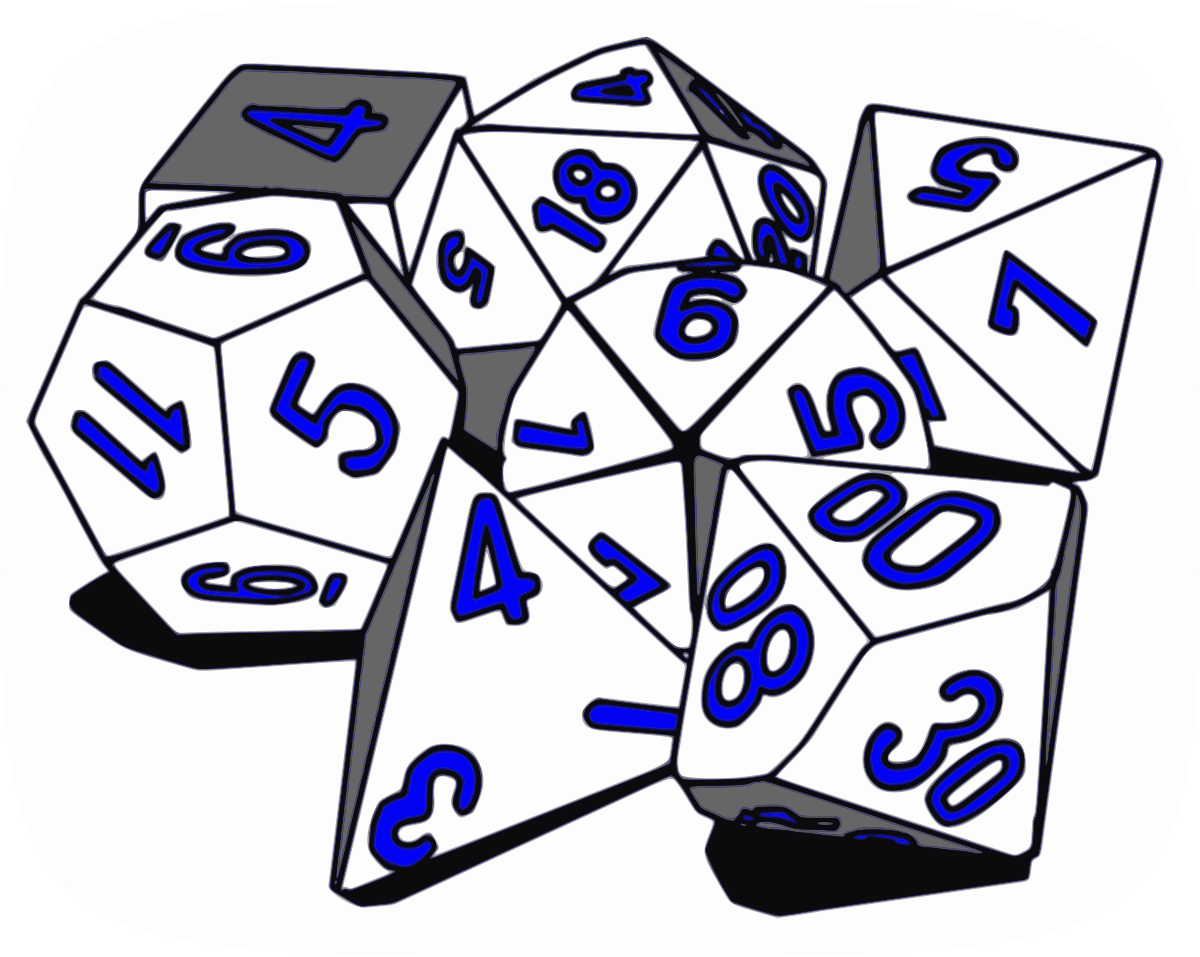
\includegraphics[width=\columnwidth]{Sections/Introduction - Basic Game Concepts - Dice}

\example{Marcie has to roll to see if Black Leaf (her rogue character) has successfully climbed a sheer wall or not. In order to do this, she needs to roll d100 and get less than or equal to Black Leaf’s Climb Walls ability. Black Leaf’s ability is 87, so Marcie needs to roll an 87 or lower.

Marcie has a red d10 and a white d10. She has declared at the beginning of the game that she will always use the red d10 as tens and the white d10 as units, so she doesn’t need to re-specify this each time she rolls.

She rolls both d10s, and gets a 9 on the red die and a 0 on the white die. Therefore, her d100 roll is 90, which is more than 87 so Black Leaf has failed to climb the wall. Had the die rolls been the other way around (0 on red and 9 on white), her d100 roll would have been 09 and she would have succeeded.}

\subsubsection{Multiple Dice}
Often, you will need to roll more than one die at the same time. In this case, there will be a number before the ‘d’ as well as after it.

The number before the ‘d’ shows how many dice must be rolled. If this number is one then it is sometimes skipped.

When rolling multiple dice in this way, simply add the numbers rolled on each die together in order to generate a single result.

Therefore, if you are told to roll “3d6”, you should roll three six sided dice and add the numbers rolled together. If you are told to roll “2d8”, you should roll two eight sided dice and add the numbers rolled together. If you are told to roll “d4”, then this is exactly the same as being told to roll “1d4”, and you should roll a single four sided die.

\subsubsection{Dice Modifiers}
Sometimes rolls will have additional modifiers. These are straightforward and are simply added or subtracted from the total rolled.

For example, if instructed to roll “2d6+4”, roll two six sided dice and add the numbers rolled together; and then add four to the result. If instructed to roll “1d8-1”, roll a single eight sided die and subtract one from the number rolled.

\section{How Do You Play?}
Before starting, one person will decide to be the Game Master. That person is responsible for establishing a setting for the game (either creating their own or using a published one). The other players create characters that live in that setting. The characters have a set of abilities which represent their capabilities; for example how strong they are or what sort of magic they are capable of using.

Then, normal play consists of the Game Master describing the situation that the characters find themselves in, and the players responding by telling the Game Master what their characters are doing.

In many situations, this is all that is required, but to provide structure and consistency to the game, this book provides rules covering what characters can do in various situations.

Additionally, many situations involve random factors, where a character has a chance of successfully doing something (which may vary depending on their abilities) rather than being automatically successful or relying on the Game Master’s whim; for example, when fighting with monsters.

In these situations, the rules tell you which type of dice to roll and how to interpret the results.

\end{multicols*}

